%!TEX program = xelatex
\documentclass[11pt, a4paper]{article}
  \usepackage[a4paper,top=3cm,bottom=4cm,left=2.5cm,right=2.5cm]{geometry}
  \usepackage{subfig}
  \usepackage{graphicx}
  \graphicspath{{../images/}}
  \usepackage{hyperref}
  \usepackage{amsmath}
  \usepackage{braket}
  \usepackage{enumitem}
  \usepackage{multirow}
  \usepackage{mathtools}
  \usepackage{xepersian}
  \settextfont[Scale=1.2]{B Nazanin}
  \setlatintextfont[Scale=1]{Times New Roman Cyr}
  \title{\textbf{شبیه‌سازی رایانه‌ای در فیزیک}\\تمرین ششم: شبکه‌های پیچیده و مونت کارلو}
  \author{سینا معمر ۹۵۱۰۲۳۱۶}
    

\begin{document}

\maketitle
\thispagestyle{empty}


\section{\textbf{شبکه اردوش-رنی}}
کد این بخش از تمرین را در فایل
\lr{q1.py}
می‌توان مشاهده نمود.
در ابتدا باید تابع
\lr{analyse\_erdos\_renyi}
را با تعداد راس‌ها و میانگین درجه رئوس دل‌خواه صدا می‌کنیم.
روش کار این تابع به این صورت است که ابتدا تعداد یال‌های متناسب با این داده‌ها را پیدا می‌کند
و یک گراف تصادفی با تعداد رئوس و یال‌های داده شده می‌سازد.
سپس درجه رئوس و خوشگی هر راس را به دست آورده و نمودار هیستوگرام آن‌ها را رسم می‌کند.
نتایج به دست آمده را می‌توان در شکل‌های
\ref{fig:q1_500_.8}،
\ref{fig:q1_500_1}
و
\ref{fig:q1_500_8}
مشاهده نمود.
\\
همان‌طور که دیده می‌شود، با افزایش
$\braket{k}$
قله‌ی منحنی توزیع درجه رئوس نیز در نمودار به سمت راست حرکت می‌کند و افزایش می‌یابد و این مقدار تقریبا برابر با همان‌
$\braket{k}$
داده شده است.
علاوه بر آن به دلیل افزایش تعداد
$k$
های محتمل در شبکه، داده‌های بیش‌تری خواهیم داشت و نمودار حول
$\braket{k}$
هموارتر می‌شود.
\\
در مورد توزیع خوشگی نکته‌ی قابل توجه،
تیز بودن منحنی به دست آمده است.
به این صورت که حتی برای
$\braket{k}$
های بزرگ نیز توزیع خوشگی پهنای بسیار کمی دارد.
برای
$\braket{k} = 0.8,\ 1$
این مقدار تقریبا همیشه صفر است ولی با افزایش میانگین درجه رئوس مشاهده می‌کنیم که قدری پهنای آن زیاد شده
و هم‌چنین قله‌ی آن به سمت راست شروع به حرکت می‌کند.
\\
اگر بخواهیم برای ذخیره‌سازی شبکه از ماتریس مجاورت استفاده کنیم، به یک ماتریس
$N \times N$
نیاز خواهیم داشت. از آن جایی هم که گراف وزن‌دار نیست، هر درایه تنها مقادیر
$1$
و
$0$
را می‌تواند داشته باشد پس تنها یک بیت نیاز است.
در نتیجه برای ذخیره‌سازی شبکه به صورت ماتریس مجاورت به
\begin{equation}
  \text{\lr{memory}} = N^2 \ \text{\lr{bits}} = \frac{N^2}{8} \ \text{\lr{bytes}}
\end{equation}

حافظه نیاز است.
\\
اگر بخواهیم از لیست مجاورت استفاده کنیم، باید دو برابر تعداد یال‌ها ($m$)
حافظه داشته باشیم. برای یک ماشین
$32-bit$
ای به

\begin{equation}
  \begin{cases}
    \text{\lr{memory}} = 2m \times 32 \ \text{\lr{bits}} = 8m \ \text{\lr{bytes}} \\
    \braket{k} = \frac{2m}{N} \Rightarrow m = \frac{\braket{k}N}{2}
  \end{cases}
  \Rightarrow
  \text{\lr{memory}} = 4N\braket{k} \text{\lr{bytes}}
\end{equation}

حافظه نیاز است.
\\
برای ذخیره کردن با استفاده از لیست یال‌ها نیز به
$2m$
خانه‌ی حافظه نیاز داریم. در نتیجه همانند لیست مجاورت برای یک ماشین
$32-bit$
ای به
\begin{equation}
  \text{\lr{memory}} = 4N\braket{k} \text{\lr{bytes}}
\end{equation}

حافظه نیاز است.
\\
برای جمع‌بندی و برای این سه شبکه‌ی داده شده می توان به جدول
\ref{tab:q1_memory}
مراجعه کرد.

\begin{table}[h!]
  \centering
  \begin{tabular}{|c|c|c|c|c|c|}
    \hline
    \lr{edge list} & \lr{adjacency list} & \lr{adjacency matrix} & \multicolumn{3}{c|}{}   \\ \hline
    $4N\braket{k} \text{\lr{bytes}}$ & $4N\braket{k} \text{\lr{bytes}}$ & $\frac{N^2}{8} \ \text{\lr{bytes}}$ & $m = \frac{N\braket{k}}{2}$ & $\braket{k}$ &          $N$         \\ \hline
    $1.6 \text{\lr{ kilobytes}}$ & $1.6 \text{\lr{ kilobytes}}$ & $31.25 \text{\lr{ kilobytes}}$ & $200$ & $0.8$ & \multirow{3}{*}{$500$} \\ \cline{1-5}
    $2 \text{\lr{ kilobytes}}$ & $2 \text{\lr{ kilobytes}}$ & $31.25 \text{\lr{ kilobytes}}$ & $250$ & $1$ &                   \\ \cline{1-5}
    $16 \text{\lr{ kilobytes}}$ & $16 \text{\lr{ kilobytes}}$ & $31.25 \text{\lr{ kilobytes}}$ & $2000$ & $8$ &                   \\ \hline
  \end{tabular}
  \caption{میزان حافظه‌ی مورد نیاز برای روش‌های ذخیره‌سازی متفاوت}
  \label{tab:q1_memory}
\end{table}

\begin{figure}[h!]
  \begin{tabular}{|c|c|c|}
    \hline
    \subfloat[گراف شبکه]{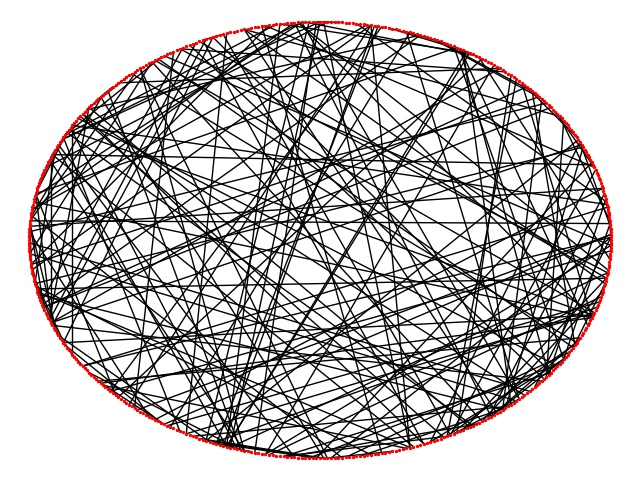
\includegraphics[width=.32\textwidth]{q1_500_0.8_graph.jpg}} &
    \subfloat[منحنی توزیع درجه رئوس]{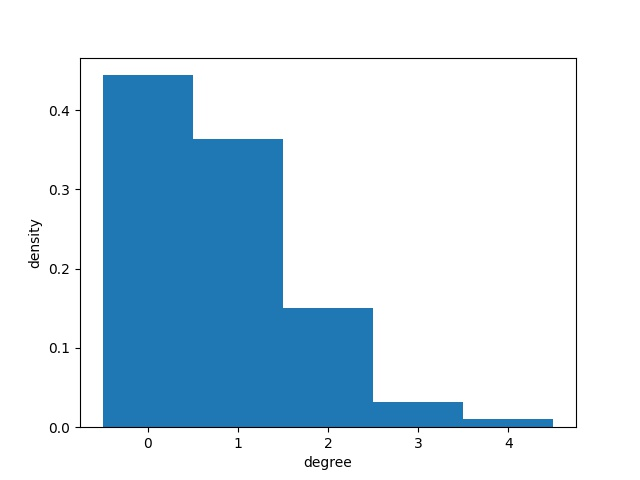
\includegraphics[width=.32\textwidth]{q1_500_0.8_degree.jpg}} &
    \subfloat[منحنی توزیع خوشگی رئوس]{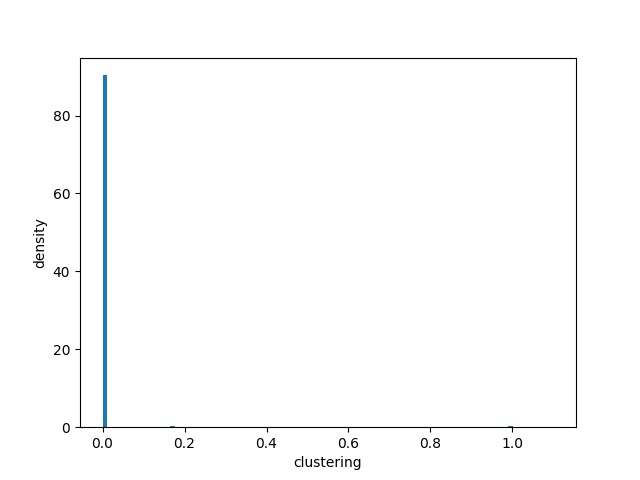
\includegraphics[width=.32\textwidth]{q1_500_0.8_clustering.jpg}} \\
    \hline
  \end{tabular}
  \caption{شبکه‌ی اردوش-رنی با $N = 500$ و $\braket{k} = 0.8$}
  \label{fig:q1_500_.8}
\end{figure}

\begin{figure}[h!]
  \begin{tabular}{|c|c|c|}
    \hline
    \subfloat[گراف شبکه]{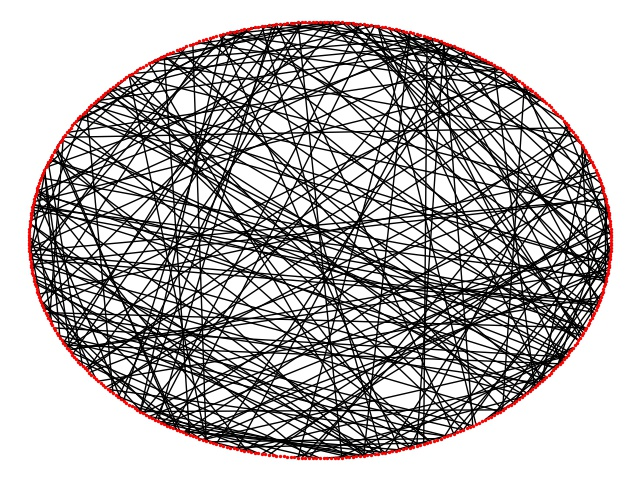
\includegraphics[width=.32\textwidth]{q1_500_1_graph.jpg}} &
    \subfloat[منحنی توزیع درجه رئوس]{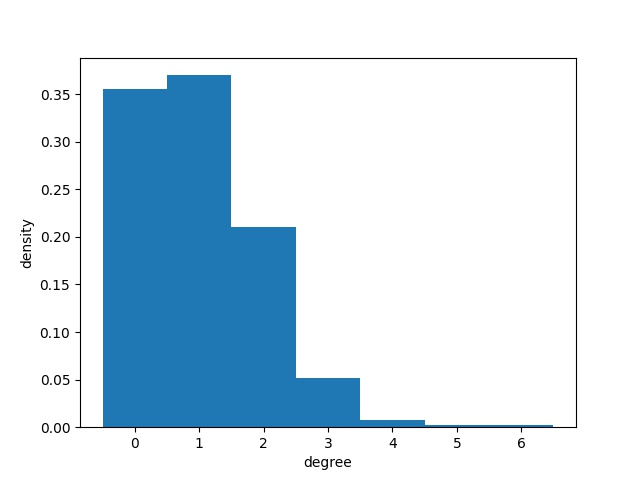
\includegraphics[width=.32\textwidth]{q1_500_1_degree.jpg}} &
    \subfloat[منحنی توزیع خوشگی رئوس]{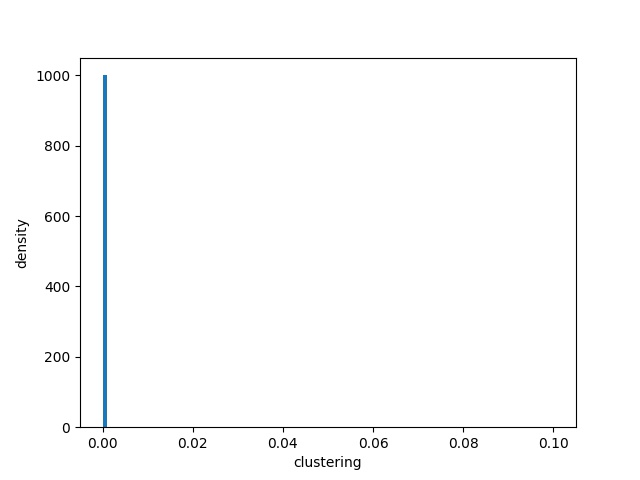
\includegraphics[width=.32\textwidth]{q1_500_1_clustering.jpg}} \\
    \hline
  \end{tabular}
  \caption{شبکه‌ی اردوش-رنی با $N = 500$ و $\braket{k} = 1$}
  \label{fig:q1_500_1}
\end{figure}

\begin{figure}[h!]
  \begin{tabular}{|c|c|c|}
    \hline
    \subfloat[گراف شبکه]{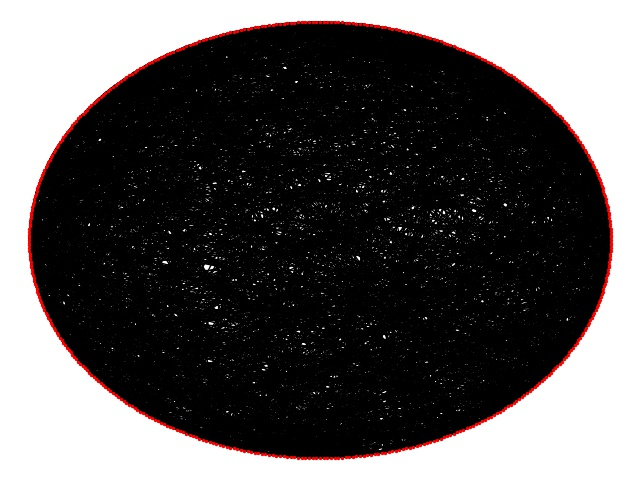
\includegraphics[width=.32\textwidth]{q1_500_8_graph.jpg}} &
    \subfloat[منحنی توزیع درجه رئوس]{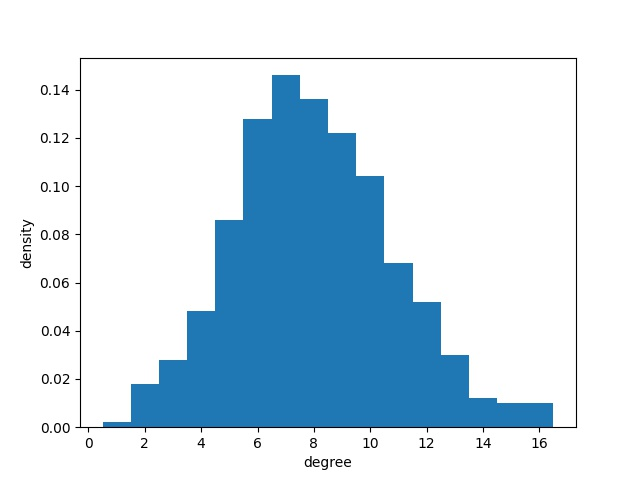
\includegraphics[width=.32\textwidth]{q1_500_8_degree.jpg}} &
    \subfloat[منحنی توزیع خوشگی رئوس]{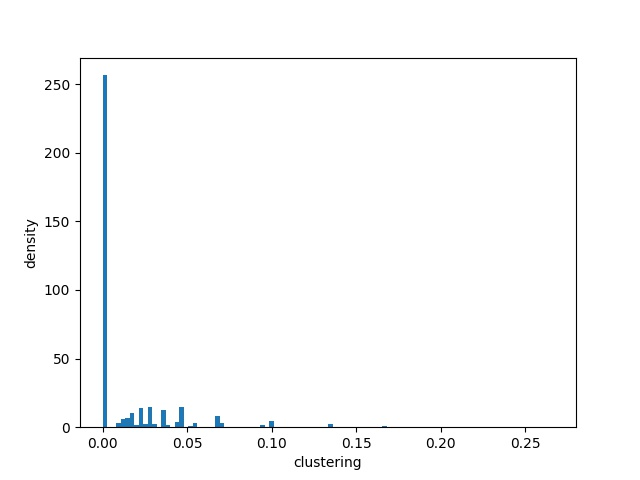
\includegraphics[width=.32\textwidth]{q1_500_8_clustering.jpg}} \\
    \hline
  \end{tabular}
  \caption{شبکه‌ی اردوش-رنی با $N = 500$ و $\braket{k} = 8$}
  \label{fig:q1_500_8}
\end{figure}


\section{\textbf{انتگرال‌گیری مونت کارلو}}
کد این بخش از تمرین را در فایل
\lr{q2.py}
می‌توان مشاهده نمود.
در ابتدا باید تابع
\lr{monte\_carlo}
را فراخوانی کنیم.
این تابع حد بالا و پایین انتگرال، تابع تولید اعداد تصادفی،
تابع هوشمند و تعداد نمونه‌ها را به عنوان ورودی می‌گیرد.
سپس تابع انتگرال را از تقسیم تابع داده شده به تابع هوشمند می‌سازد.
در نهایت نیز به تعداد نمونه‌های داده شده، با استفاده از تابع تولید اعداد تصادفی داده شده، اعداد تصادفی می‌سازیم و
مقدار تابع انتگرال را در آن نقاط حساب می‌کنیم.
سپس میانگین آن‌ها را ضرب در ضریب اسکیل به عنوان مقدار انتگرال و انحراف نسبی آن را نیز به عنوان خطای آماری بر می‌گردانیم.
این تابع را به صورت ساده و با دو تابع هوشمند متفاوت و با تعداد نمونه‌های مختلف  برای انتگرال 
$\int_0^2 e^{-x^2}$
صدا می‌کنیم.
نتایج به دست آمده را در جداول
\ref{tab:q2_integral_simple}،
\ref{tab:q2_integral_e_x}
و
\ref{tab:q2_integral_1_x_2}
می‌توان مشاهده نمود.
\\
همان طور که دیده می‌شود،
با افزایش تعداد نمونه‌ها، زمان اجرا و دقت مقدار به دست آمده هر دو افزایش می‌یابند که مطابق با انتظار ما است.
علاوه بر آن مشاهده می‌شود که زمان اجرا به طور خطی افزایش پیدا می‌کند که با توجه به اینکه صرفا در تابع مورد نظر
به تعداد نمونه‌ها داده شده باید مقدار تابع انتگرال را محاسبه کنیم، پس نتیجه‌ای منطقی است.
همان طور که انتظار داشتیم، زمان اجرا در حالت نمونه‌برداری ساده، کم‌تر از نمونه‌برداری هوشمند است
که علت آن وجود محاسبات اضافه‌تر برای به دست آوردن اعداد تصادفی با توزیع مورد‌نظر و محاسبه‌ی مقدار تابع هوشمند است.
ولی در ازای آن دقت بالاتری را در زمان کم‌تر به دست می‌آوریم.
برای نمونه می‌توان به مقدار خطای واقعی
$0.0006$
نگاه کرد.
برای نمونه‌برداری ساده،
$2.0$
ثانیه و برای نمونه‌برداری هوشمند،
$0.41$
ثانیه زمان برده است.
در نتیجه اگر چه در نمونه برداری هوشمند در تعداد نمونه‌های ثابت به زمان بیش‌تری نیاز است
ولی در تعداد نمونه‌های کم‌تری و در نتیجه در زمان کم‌تر می‌توان به دقت مطلوب رسید.

\begin{table}[h!]
  \centering
  \begin{tabular}{|c|c|c|c|c|c|}
    \hline
    \multirow{2}{*}{\text{مقدار واقعی}} & \multicolumn{4}{c|}{\lr{Simple Sampling}} & \multirow{2}{*}{$N$} \\ \cline{2-5}
    &   \text{زمان اجرا}    &   \text{خطای واقعی}    &   \text{خطای آماری}   &   \text{مقدار}   &                                \\ \hline
    \multirow{6}{*}{$0.882081$} &    $0.00015$   &   $-0.038$    &    $0.02$   &   $0.92$   &     $10^3$        \\ \cline{2-6}
    &    $0.00030$   &   $-0.014$    &    $0.007$   &   $0.896$   &     $10^4$        \\ \cline{2-6}
    &   $0.0030$    &    $-0.002$   &   $0.002$    &   $0.884$   &     $10^5$        \\ \cline{2-6}
    &   $0.022$    &     $0.001$  &   $0.0007$    &   $0.8809$   &     $10^6$        \\ \cline{2-6}
    &   $0.21$    &      $0.0002$ &   $0.0002$    &  $0.8819$    &     $10^7$        \\ \cline{2-6}
    &   $2.0$    &     $0.00006$  &   $0.00007$    &  $0.88214$    &     $10^8$        \\ \hline
  \end{tabular}
  \caption{مقایسه مقدار انتگرال، خطای آماری، خطای واقعی و زمان اجرای مونت کارلو برای $\int_0^2 e^{-x^2}$ با نمونه‌برداری ساده}
  \label{tab:q2_integral_simple}
\end{table}

\begin{table}[h!]
  \centering
  \begin{tabular}{|c|c|c|c|c|c|}
    \hline
    \multirow{3}{*}{\text{مقدار واقعی}} & \multicolumn{4}{c|}{\lr{Important Sampling}} & \multirow{3}{*}{$N$} \\ \cline{2-5}
    & \multicolumn{4}{c|}{$g(x) = e^{-x}$} &                   \\ \cline{2-5}
    &   \text{زمان اجرا}    &   \text{خطای واقعی}    &   \text{خطای آماری}   &   \text{مقدار}   &                                \\ \hline
    \multirow{6}{*}{$0.882081$} &    $0.0001$   &   $0.009$    &    $0.008$   &   $0.873$   &     $10^3$        \\ \cline{2-6}
    &    $0.00036$   &   $-0.002$    &    $0.003$   &   $0.884$   &     $10^4$        \\ \cline{2-6}
    &   $0.0038$    &    $-0.0004$   &   $0.0008$    &   $0.8825$   &     $10^5$        \\ \cline{2-6}
    &   $0.037$    &     $0.00008$  &   $0.0003$    &   $0.8820$   &     $10^6$        \\ \cline{2-6}
    &   $0.41$    &      $0.00006$ &   $0.00008$    &  $0.88202$    &     $10^7$        \\ \cline{2-6}
    &   $3.7$    &     $-0.00003$  &   $0.00003$    &  $0.88211$    &     $10^8$        \\ \hline
  \end{tabular}
  \caption{مقایسه مقدار انتگرال، خطای آماری، خطای واقعی و زمان اجرای مونت کارلو برای $\int_0^2 e^{-x^2}$ و با تابع هوشمند $g(x) = e^{-x}$}
  \label{tab:q2_integral_e_x}
\end{table}

\begin{table}[h!]
  \centering
  \begin{tabular}{|c|c|c|c|c|c|}
    \hline
    \multirow{3}{*}{\text{مقدار واقعی}} & \multicolumn{4}{c|}{\lr{Important Sampling}} & \multirow{3}{*}{$N$} \\ \cline{2-5}
    & \multicolumn{4}{c|}{$g(x) = \frac{1}{1 + x^2}$} &                   \\ \cline{2-5}
    &   \text{زمان اجرا}    &   \text{خطای واقعی}    &   \text{خطای آماری}   &   \text{مقدار}   &                                \\ \hline
    \multirow{6}{*}{$0.882081$} &    $0.0001$   &   $-0.009$    &    $0.009$   &   $0.891$   &     $10^3$        \\ \cline{2-6}
    &    $0.00047$   &   $-0.004$    &    $0.003$   &   $0.886$   &     $10^4$        \\ \cline{2-6}
    &   $0.0051$    &    $-0.00002$   &   $0.0009$    &   $0.8821$   &     $10^5$        \\ \cline{2-6}
    &   $0.050$    &     $0.0003$  &   $0.0003$    &   $0.8818$   &     $10^6$        \\ \cline{2-6}
    &   $0.55$    &      $0.00002$ &   $0.00009$    &  $0.88206$    &     $10^7$        \\ \cline{2-6}
    &   $5.1$    &     $-0.00001$  &   $0.00003$    &  $0.88209$    &     $10^8$        \\ \hline
  \end{tabular}
  \caption{مقایسه مقدار انتگرال، خطای آماری، خطای واقعی و زمان اجرای مونت کارلو برای $\int_0^2 e^{-x^2}$ و با تابع هوشمند $g(x) = \frac{1}{1 + x^2}$}
  \label{tab:q2_integral_1_x_2}
\end{table}


\section{\textbf{انتگرال چندگانه}}
کد این بخش از تمرین را در فایل
\lr{q3.py}
می‌توان مشاهده نمود.
در ابتدا باید تابع
\lr{compute\_com}
را با شعاع، تابع چگالی و تعداد نمونه‌های دل‌خواه صدا کنیم.
روش کار این تابع به این صورت است که ابتدا به تعداد نمونه‌های داده شده، نقاط تصادفی در
$x$،
$y$
و
$z$
انتخاب می‌کند.
سپس اندیس آن‌هایی را که در داخل کره می‌افتند را به دست می‌آورد و آن‌ها را به عنوان نقاط تصادفی نهایی ذخیره می‌کند.
در آخر نیز تابع چگالی را با این نقاط صدا کرده و چگالی‌های به دست آمده را در مختصات نقاط ضرب می‌کند.
به عنوان خروجی نیز میانگین این مقادیر را به عنوان مختصات مرکز جرم و
انحراف معیار نسبی آن‌ها را به عنوان خطای آماری این مقادیر بر می‌گرداند.
نتایج به دست آمده برای شعاع
$5$
و تعداد
$10^8$
به صورت زیر است:
\begin{equation}
  \begin{cases}
    X = 0.0000 \pm 0.0002 \\
    Y = 0.0005 \pm 0.0002 \\
    Z = 0.3328 \pm 0.0002 \\
  \end{cases}
\end{equation}


\section{\textbf{متروپولیس}}
کد این بخش از تمرین را در فایل
\lr{q4.py}
می‌توان مشاهده نمود.
در ابتدا باید
\lr{object}
از کلاس
\lr{Metropolis}
با تابع توزیع دل‌خواه بسازیم.
سپس تابع
\lr{generate}
را روی آن با زمان، مکان اولیه و طول قدم دل‌خواه صدا می‌کنیم.
روش کار این تابع به این صورت است که به اندازه‌ی زمان داده شده، 
عدد تصادفی دل‌خواه برای تعیین مکان نقطه‌ی بعدی و احتمال حرکت در آن زمان تولید می‌کنیم.
سپس روی زمان داده شده پیمایش کرده و در مرحله با استفاده از انتخاب متروپولیس، می‌بینیم که آیا باید حرکت کنیم یا نه.
به این ترتیب اعداد تصادفی جدید را به دست می‌آوریم.
هم‌چنین در هر مرحله اگر جابجا بشویم، مقدار متغیر
\lr{acceptance\_count}
را یکی زیاد می‌کنیم.
در نهایت نیز می‌توانیم نرخ قبولی را با صدا کردن تابع
\lr{get\_acceptance\_rate}
به دست بیاوریم.
برای به دست آوردن طول هم‌بستگی نیز روی
$j$
های مختلف پیمایش کرده و برای هر کدام مقدار هم‌بستگی را محاسبه می‌کنیم.
در نهایت یک تابع نمایی را به داده‌‌های به دست آمده فیت می‌کنیم و از روی پارامتر‌های آن، طول هم‌بستگی را گزارش می‌کنیم.
نتایج به دست آمده را در جدول
\ref{tab:q4_l}
می‌توان مشاهده نمود.
همان طور که دیده می‌شود برای
$0.4 < a_r < 0.5$
کم‌ترین طول هم‌بستگی را خواهیم داشت.
پس برای اینکه در سریع‌ترین زمان به تابع توزیع دل‌خواه برسیم،
باید
$a_r$
را در این بازه تنظیم بکنیم.
در نتیجه برای نمونه می‌توانیم طول قدم‌ را
$7$
در نظر بگیریم.
در این صورت طول هم‌بستگی
$1.74$
و نرخ قبولی
$0.438$
می‌شود. پس اعداد تولید شده‌ای که با یکدیگر حداقل
$2\xi = 3.48 \approx 3$
فاصله دارند را می‌توان بدون هم‌بستگی در نظر گرفت و به عنوان اعداد تصادفی گزارش نمود.
نمودار توزیع این اعداد را در شکل‌
\ref{fig:q4_distrubation}
می‌توان مشاهده نمود.

\begin{table}[h!]
  \centering
  \begin{tabular}{|c|c|c|}
    \hline
    $\xi$ & $\Delta$ & $a_r$ \\ \hline
    $7.34$ & $31.92$ & $0.100$ \\ \hline
    $3.39$ & $15.93$ & $0.200$ \\ \hline
    $2.12$ & $10.60$ & $0.300$ \\ \hline
    $1.75$ & $7.77$ & $0.400$ \\ \hline
    $1.90$ & $5.88$ & $0.500$ \\ \hline
    $2.54$ & $4.41$ & $0.600$ \\ \hline
    $3.98$ & $3.15$ & $0.700$ \\ \hline
    $7.95$ & $2.04$ & $0.800$ \\ \hline
    $27.1$ & $1.01$ & $0.900$ \\ \hline
  \end{tabular}
  \caption{نرخ قبولی‌های مختلف و طول قدم‌ها و طول هم‌بستگی‌های متناظر با آن‌ها برای توزیع گاوسی با $\sigma = 2$، $x_0 = 0$ و با زمان $10^6$}
  \label{tab:q4_l}
\end{table}

\begin{figure}
  \centering
  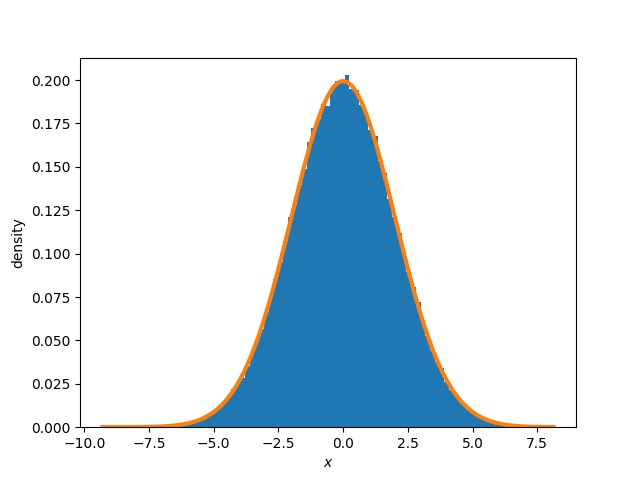
\includegraphics[width=.7\textwidth]{q4_0_1000000_7.jpg}
  \caption{تابع توزیع اعداد تصادفی تولید شده با روش متروپولیس برای توزیع گاوسی با $\sigma = 2$، $\Delta = 7$ و با $10^6$ نمونه}
  \label{fig:q4_distrubation}
\end{figure}


\end{document}
